\documentclass[lualatex,ja=standard]{bxjsarticle}

\setpagelayout{noheadfoot,top=1cm,bottom=1cm,left=2cm,right=2cm}

% タイトル情報(必要に応じて編集)
\title{実験レポートタイトル}
\author{作成者名}
\date{\today}

% パッケージ類
\usepackage{graphicx}
\usepackage{amsmath}
\usepackage{amssymb}
\usepackage{caption}
\usepackage{subcaption}
\usepackage{siunitx}
\usepackage{booktabs}
\usepackage{pdfpages}
\usepackage{enumitem}
\usepackage{titlesec}
\usepackage{luatexja-fontspec}
\usepackage{ascmac}
\usepackage{hyperref}
\usepackage{xspace}

% フォント
\setmainjfont{IPAexMincho} 
\AtBeginDocument{%
  \fontsize{10.5pt}{16pt}\selectfont
}

% 樹形図
\usepackage{tikz}
\usetikzlibrary{graphs, graphdrawing, arrows.meta, calc}
\usegdlibrary{trees}  % trees 用ライブラリ

% セクションスタイル
\newcommand{\mysectionstyle}[2]{%
  \sffamily         % 欧文・数字→サンセリフ
  \gtfamily         % 日本語→ゴシック
  \bfseries
  \fontsize{#1}{#2}\selectfont
}

% セクションのスタイル
\titleformat{\section}
  {\mysectionstyle{12pt}{16pt}}
  {\mysectionstyle{12pt}{16pt}\thesection.}
  {0.7em}{}
\titlespacing*{\section}{0em}{1em}{0em}

% サブセクションのスタイル
\titleformat{\subsection}
  {\mysectionstyle{10.5pt}{16pt}}
  {\mysectionstyle{10.5pt}{16pt}\thesubsection.}
  {0.7em}{}
\titlespacing*{\subsection}{0em}{0.5em}{0em}

% サブサブセクションのスタイル
\titleformat{\subsubsection}
  {\mysectionstyle{10.5pt}{12pt}}
  {\mysectionstyle{10.5pt}{12pt}\thesubsubsection.}
  {0em}{}
\titlespacing*{\subsubsection}{0em}{0.5em}{0em}

% パラグラフのスタイル
\titleformat{\paragraph}
  {\mysectionstyle{10.5pt}{12pt}}
  {\mysectionstyle{10.5pt}{12pt}\theparagraph.} 
  {0em}{}
\titlespacing*{\paragraph}{0em}{0em}{0em}

% サブパラグラフのスタイル
\titleformat{\subparagraph}
  {\mysectionstyle{8pt}{12pt}}
  {\mysectionstyle{8pt}{12pt}\thesubparagraph.}
  {0em}{}
\titlespacing*{\subparagraph}{0em}{0em}{0em}

% 和文キャプション
\renewcommand{\figurename}{図}
\renewcommand{\tablename}{表}
\renewcommand{\refname}{参考文献}

% autoref の和文化
\renewcommand*{\figureautorefname}{図}
\renewcommand*{\tableautorefname}{表}
\renewcommand*{\equationautorefname}{式}
\renewcommand*{\subfigureautorefname}{図}

\captionsetup[subfigure]{labelformat=simple}
\renewcommand*{\thesubfigure}{(\alph{subfigure})}

% ブラケット付き単位の設定
\NewDocumentCommand{\sibr}{m}{\,\text{[\si{#1}]}} 

% リンクの色設定
\hypersetup{
  colorlinks=true,
  linkcolor=black,
  citecolor=black,
  urlcolor=black
}

% 段落設定
\setlength{\parskip}{0.5em}
\setlength{\parindent}{1em}
\makeatletter
\AtBeginDocument{
  \let\@afterindentfalse\@afterindenttrue
}
\makeatother

\begin{document}
\pagestyle{empty}

% 表紙(wordから出力した表紙をcover/BN.pdfに保存)
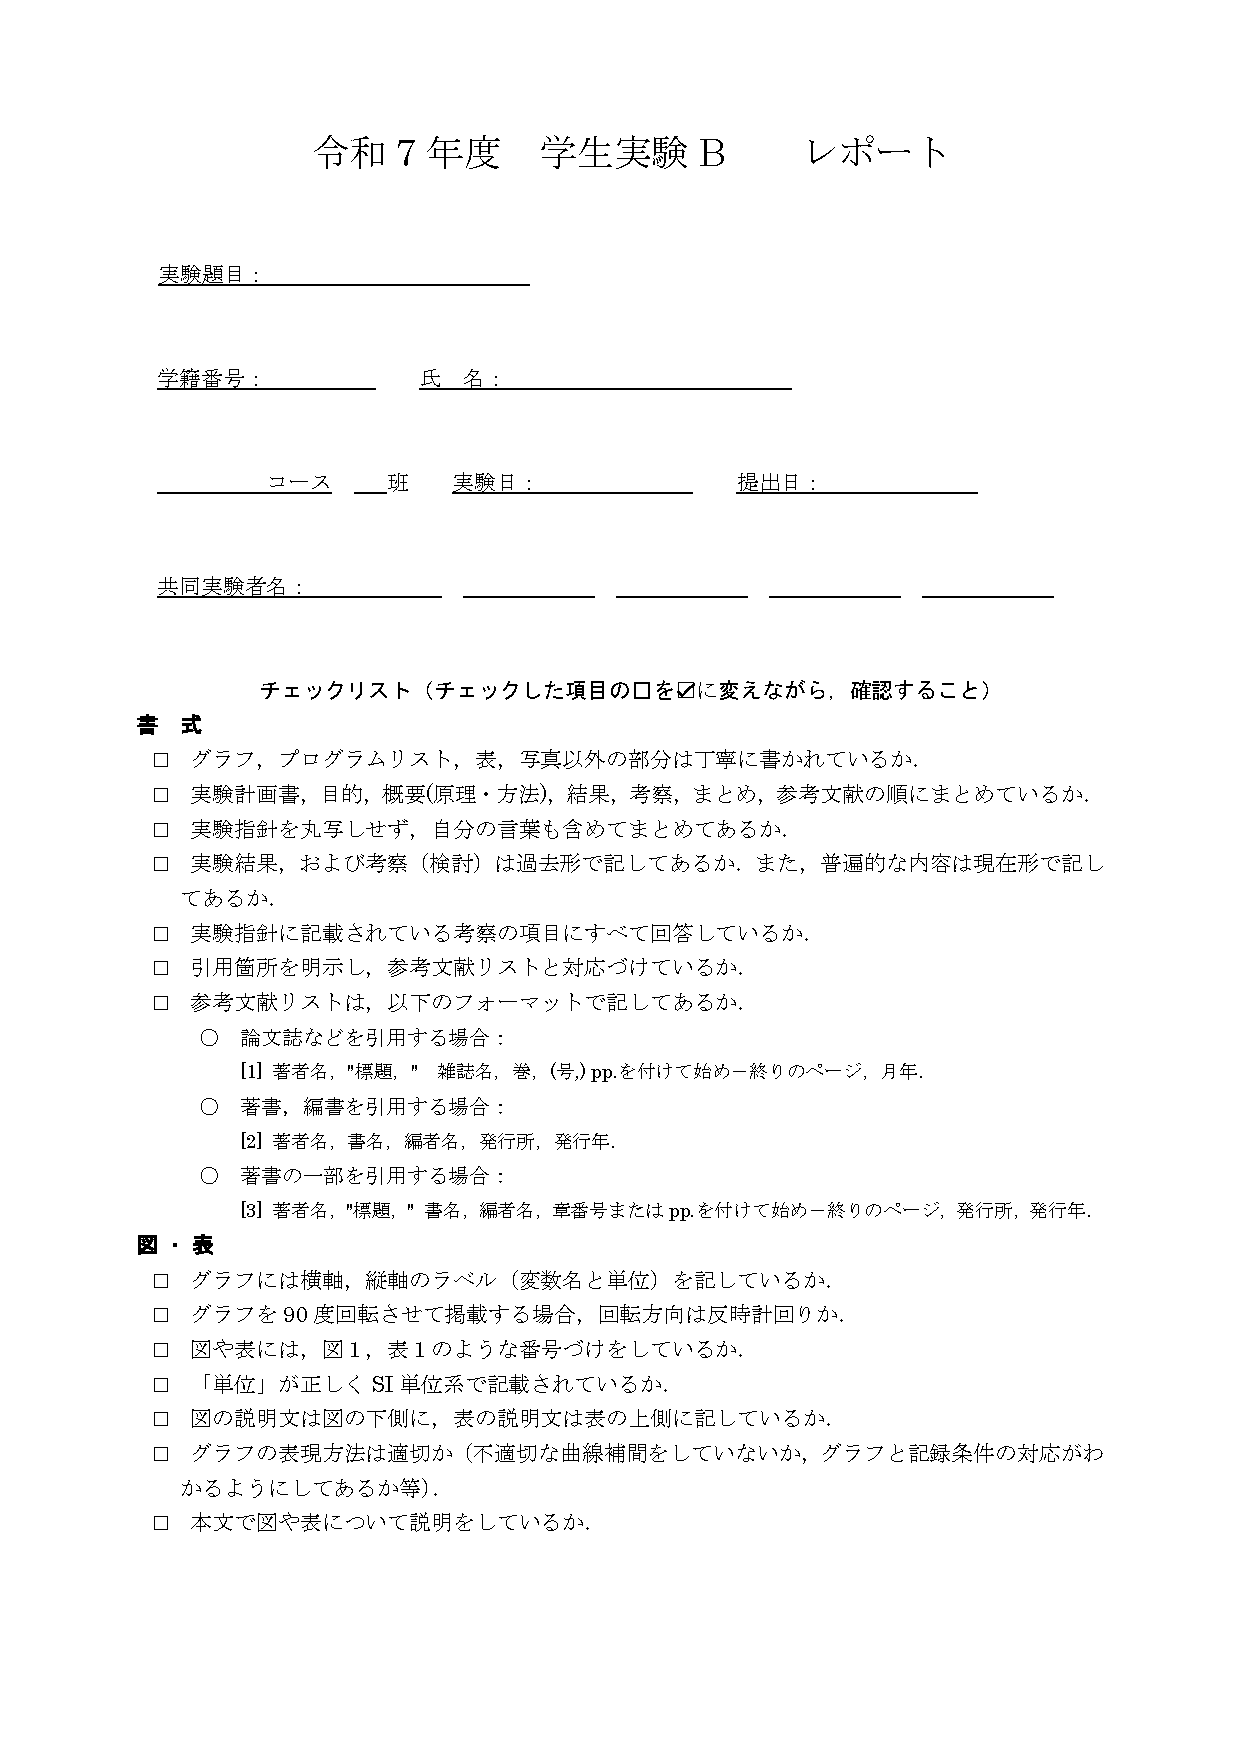
\includepdf[pages=1]{cover/BN.pdf}

\section{実験の目的}

本実験の目的をここに記述する.

\section{原理}

実験の理論的背景を簡潔に記述する.樹形図は\autoref{fig:tree-diagram}のように作成する.ChatGPTを使用して作成すると良い.

\begin{figure}[htbp]
  \centering
  % 必要に応じてTikZ図を編集または削除
  \begin{tikzpicture}[font=\normalsize, node distance=3cm and 2cm, every node/.style={draw=none, anchor=west}, >={Latex}]
    \node (root) at (0,0) {現象A};
    \node (child1) at ($(root)+(4,0.5)$) {要因1};
    \node (child2) at ($(root)+(4,-0.5)$) {要因2};
    \draw[->] (root.east) -- (child1.west);
    \draw[->] (root.east) -- (child2.west);
  \end{tikzpicture}
  \caption{現象の分類例}
  \label{fig:tree-diagram}
\end{figure}

\section{実験の方法}

\subsection*{[使用器具]}

\begin{itemize}
  \item 使用器具1
\end{itemize}

\subsection{実験概要}

ここに全体の手順や測定方法の概要を記述する.

\subsection{個別手順}

\subsubsection*{[手順]}

\begin{enumerate}
  \item 装置の初期設定
  \item 測定値の取得
  \item 注意点や補足説明(\textbf{安全注意}など)
\end{enumerate}

\section{実験結果}

結果をまとめたグラフなどを\autoref{fig:example-graph}のように挿入する.

\begin{figure}[htbp]
  \centering
  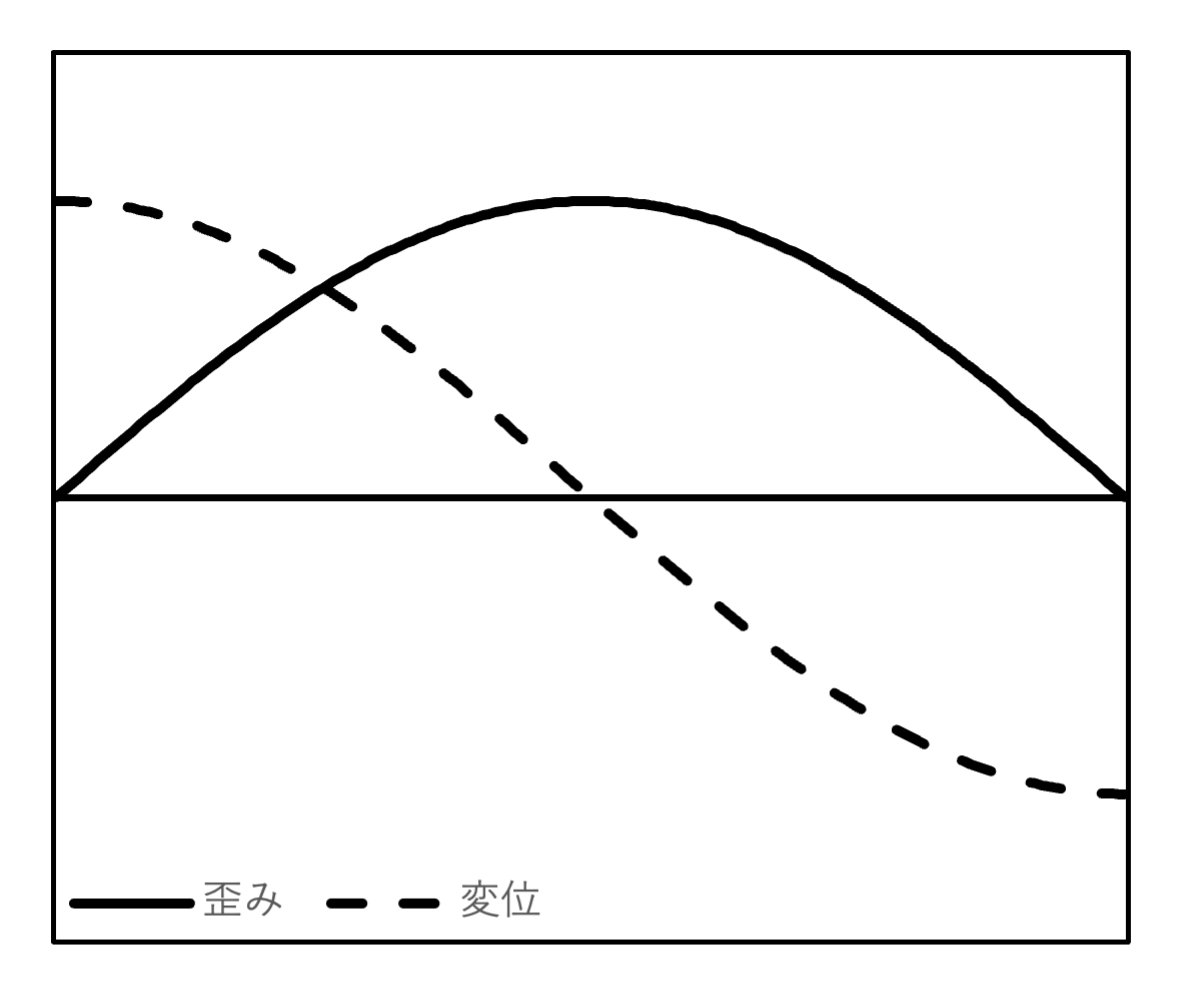
\includegraphics[width=0.4\textwidth]{img/BN/graph.png}
  \caption{グラフ例}
  \label{fig:example-graph}
\end{figure}

結果をまとめた表などは\autoref{tab:example-table}のように挿入する.

\begin{table}[htbp]
  \centering
  \caption{測定結果の例}
  \label{tab:example-table}
  \begin{tabular}{cccc}
    \toprule
    条件1 & 条件2 & 条件3 & 条件4 \\
    \midrule
    値1 & 値2 & 値3 & 値4 \\
    \bottomrule
  \end{tabular}
\end{table}

図を横並びにするには,\autoref{fig:example-double-graph}のように挿入する.

\begin{figure}[htbp]
  \centering
  \begin{subfigure}{0.48\linewidth}
    \centering
    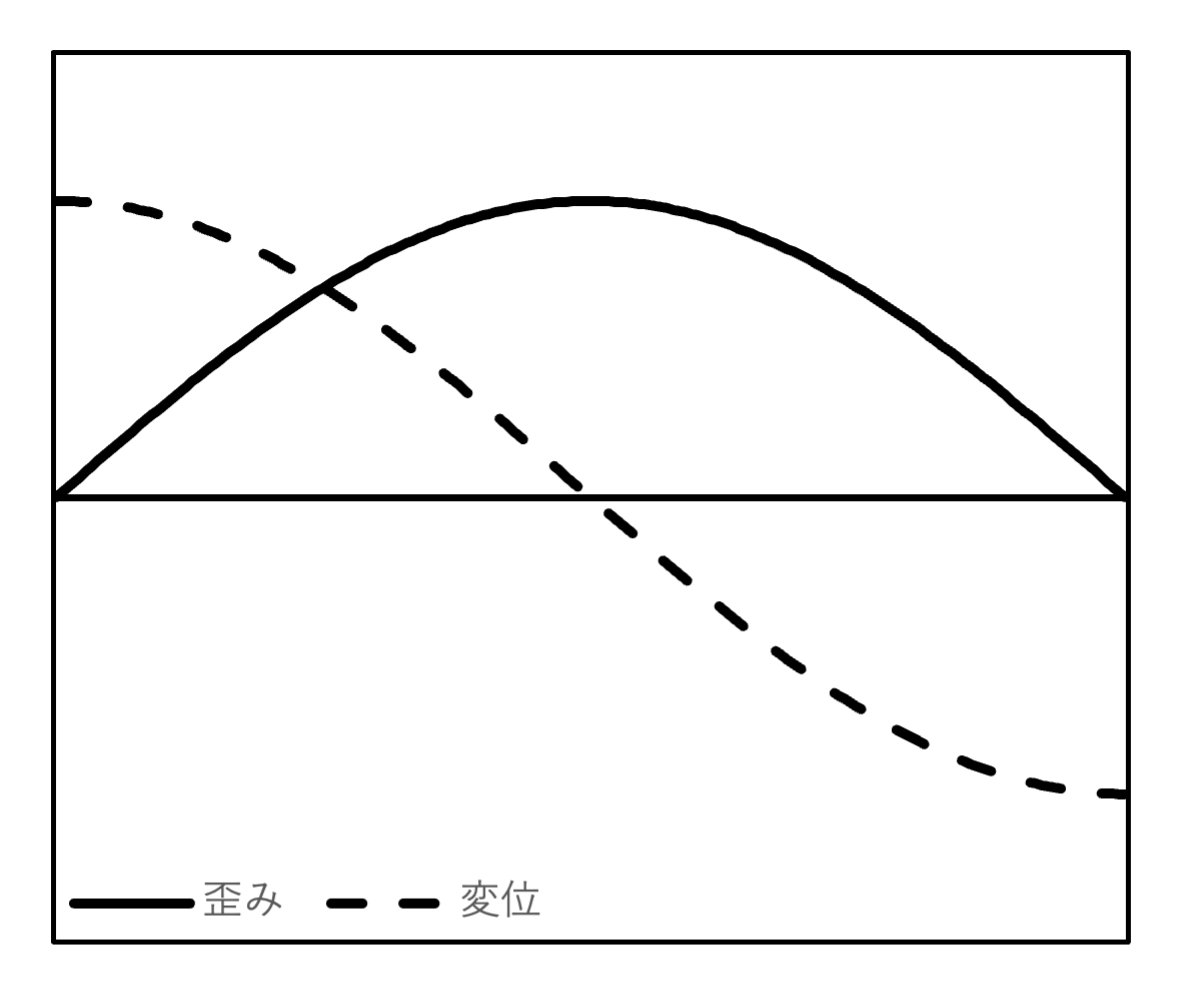
\includegraphics[width=\linewidth]{img/BN/graph.png}
    \caption{グラフ1}
    \label{fig:example-double-graph-1}
  \end{subfigure}
  \hfill
  \begin{subfigure}{0.48\linewidth}
    \centering
    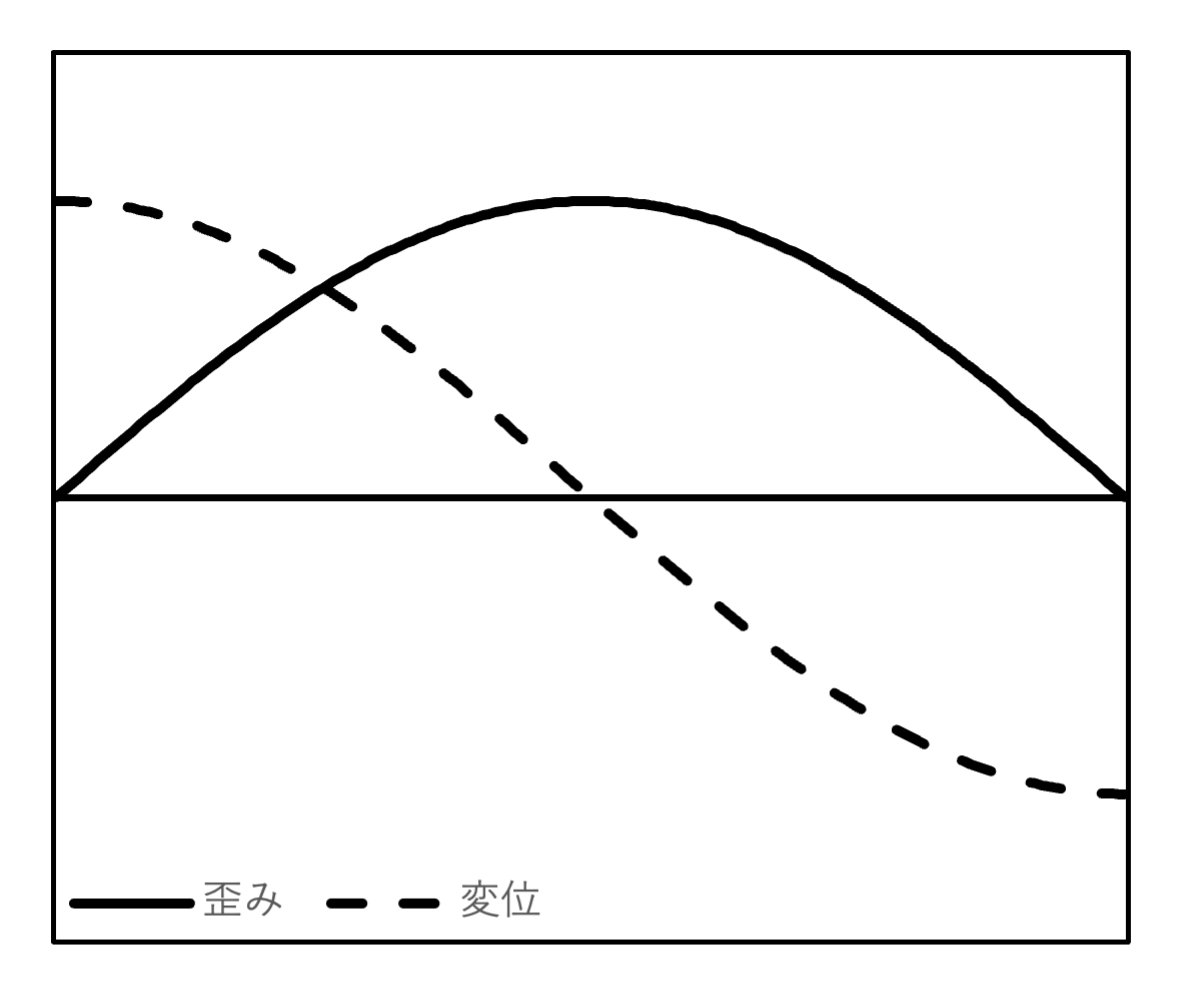
\includegraphics[width=\linewidth]{img/BN/graph.png}
    \caption{グラフ2}
    \label{fig:example-double-graph-2}
  \end{subfigure}

  \caption{横並びのグラフ}
  \label{fig:example-double-graph}
\end{figure}

測定結果の計算式は\autoref{eq:line}のように挿入する.

\begin{equation}
  y = a x + b \sibr{\meter\per\second}
  \label{eq:line}
\end{equation}

\section{考察}

実験結果に基づいて考察を記述する.たとえば,傾向の説明,理論との一致・不一致,実験誤差の要因などを検討する.

\section{結論}

実験全体の要点を簡潔にまとめる.たとえば,

\begin{itemize}
  \item 結果から得られる一般的な知見
  \item 今後の課題や応用可能性
\end{itemize}

\section*{<参考文献>}

\begin{enumerate}[label={[\arabic*]}]
  \item 教科書を参考文献とする場合の書式:\\
  著者:書物名,頁(単ページの場合 p. OO,複数ページの場合 pp. OO--OO),出版社(年).

  \item 論文誌を参考文献とする場合の書式:\\
  著者:“論文題目,” 雑誌名,巻(vol. OO または OO巻),論文頁(年).

  \item 二村忠元:電気磁気学,電子・通信・電気工学基礎講座1,p. 56, 丸善(1972).

  \item K. F. Schrum, S. H. Ko, and D. Ben-Amotz: “Description and theory of a fiber-optic confocal and super-focal Raman microspectrometer,” Appl. Spectrosc., vol. 50, pp. 1150–1155 (1996).
\end{enumerate}

\end{document}
